\documentclass{oblivoir}
\usepackage{fapapersize}
\usefapapersize{*,*,30mm,*,30mm,*}

\usepackage{amsmath}
\usepackage{amsthm}
\theoremstyle{definition}
\newtheorem{exercise}{연습문제}
\newtheorem{homework}[exercise]{숙제}
\newtheorem{example}[exercise]{예제}

\usepackage{color}

\usepackage{url}

\usepackage{tikz}

\newcommand{\inv}[1]{\textcolor{blue}{\ensuremath{[{#1}]}}}

\begin{document}
\title{올바른 프로그램 작성하기}
\author{강지훈 (\url{http://sf.snu.ac.kr/jeehoon.kang})}
\maketitle

\begin{abstract}
  이 글에서는 무엇이 올바른 프로그램인지, 어떻게 체계적으로 올바른
  프로그램을 작성할 수 있을지 알아본다.  프로그래밍할 때, 올바른
  프로그램을 작성하는 것은 무엇보다도 중요한 일이다.  소프트웨어 버그에
  인한 비용은 연간 조원 단위에 이르는 것으로 알려졌기 때문이다.  따라서
  프로그램을 처음 작성할 때부터 올바른 프로그램을 작성해야만 소프트웨어
  비용을 줄일 수 있다.  이를 위한 체계적이고 표준적인 방법론인 불변식은
  70년대에 Hoare가 처음 제시했으며, 그 이후 눈부신 발전을 이루었다.  이
  글에서는 예제를 통해 불변식의 맛을 보기로 한다.
\end{abstract}

\section{들어가며}
\subsection{올바른 프로그램을 작성해야 하는 이유}
올바른 프로그램을 작성해야 하는 까닭은, 시험에서 좋은 점수를 받기
위함도 있겠지만, 궁극적으로는 신뢰할 수 있는 소프트웨어를 작성하기
위함이다.  신뢰할 수 없는 소프트웨어의 대가는 크다.  소프트웨어 버그에
인한 비용은 연간 조원 단위에 이르는 것으로 알려졌다.  이를 막기 위해,
많은 회사에서는 소프트웨어 테스터를 소프트웨어 개발자만큼이나
고용한다.

\subsection{올바른 프로그램이란 무엇인가}
그렇다면 \emph{올바른} 프로그램이란 무엇인가?  이 글에서는, 의도한
바(명세, Specification)대로 동작하는 프로그램을 올바른 프로그램이라고
정의한다.  예를 들어 정렬 함수:
\[\texttt{sort(A: int[10]): int[10]}\]
가 있을 때, 우리가 이 함수에 기대하는 바, 즉 명세는 다음과 같을
것이다:
\begin{center}모든 $\texttt{i}<\texttt{j}$에 대해,
  $\texttt{sort(A)[i]} < \texttt{sort(A)[j]}$이다.\end{center}
\noindent 위와 같이 수학적인 명세를 줬을 때, 이 명세를 만족하는
프로그램을 \emph{그 명세에 대해} 올바른 프로그램이라고 부를 수 있다.

\begin{exercise}
  위에서 언급한 정렬의 명세가:
  \begin{enumerate}
  \item 올바른가? 예
  \item ``정렬''하는 함수에 기대하는 바를 충분히 다 표현하였는가?
    아니요
  \begin{center}\texttt{sort(A)}는 \texttt{A}에서 순서만 바꾼 것이다
    (permutation이다).\end{center} 도 명세에 추가되어야 한다.

  \end{enumerate}
\end{exercise}

\begin{exercise}\label{exercise:find}
  함수 \texttt{find(x: int, A: int[10]): bool}의 명세는 다음과 같다:
  \begin{center}\texttt{x}가 \texttt{A}에 들어있으면 \texttt{true}, 아니면
    \texttt{false}를 내놓아야 한다.\end{center} 이런 함수
  \texttt{find}를 작성하라.
\end{exercise}

\subsection{올바른 프로그램을 작성하는 방법론}
위에서 프로그램이 명세에 대해 올바르다는 것이 무엇인지 정의했다.  그럼
어떻게 올바르다는 것을 \emph{확인}할 수 있을까?

가장 간단하고 현업에서 많이 쓰이는 방법은 테스트이다.  위에서 언급한
정렬 함수를 예로 든다면, 정렬 함수에 임의의 입력을 주고, 그 출력이
정렬에 대한 명세를 만족하는지 확인하는 것이다.  한 입력에 대해서만 하는
것이 아니라 충분한 자신이 생길 때까지 반복해서 테스트한다.

테스트로 작성된 프로그램이 올바르다는 것을 대강은 확인할 수는 있지만,
테스트는 어떻게 올바른 프로그램을 작성해야 하는지에 대해서는 알려주는
바가 없다.  이를 위해서는 \emph{불변식}을 사용하면 된다.  불변식이란,
프로그램의 어떤 지점에서, 프로그램의 상태가 만족해야만 하는 성질을
말한다.  예를 들어보자.
\begin{align*}
& a: \inv{} \\
\texttt{10:}& \texttt{x:=1} \\
& b: \inv{\texttt{x}=1} \\
\texttt{11:}& \texttt{y:=2} \\
& c: \inv{\texttt{x}=1 \land \texttt{y}=2} \\
\texttt{12:}& \texttt{assert(x+1=y)} \\
& d: \inv{\texttt{x}=1 \land \texttt{y}=2 \land \texttt{x}+1=\texttt{y}}
\end{align*}
\noindent 이때, $A \land B$는 ($A$ 그리고 $B$)를 의미하며, $A \lor
B$는 ($A$ 또는 $B$)를 의미한다.  프로그램 라인 사이에 있는 $[\phi]$는
그 지점에서 프로그램의 상태가 $\phi$를 만족해야 함을 의미한다.  예를
들어 10라인과 11라인 사이에서는 $\texttt{x}=1$을 만족해야 한다.

이 불변식이 정말로 옳으려면, 예를 들어 10라인과 11라인 사이에서 정말로
$\texttt{x}=1$가 성립하려면, 다음 성질을 만족해야만 한다:
\begin{enumerate}
\item $a$ 불변식 \inv{}는 아무런 조건이 없다는 뜻이다.  이때
  \texttt{10: x:=1}을 실행하고 나면, $b$ 불변식 \inv{\texttt{x}=1}을
  만족해야만 한다.
\item $b$ 불변식 \inv{\texttt{x}=1}을 만족할 때, \texttt{11: y:=2}를
  실행하고 나면, $c$ 불변식 \inv{\texttt{x}=1 \land \texttt{y}=2}을
  만족해야만 한다.
\item $c$ 불변식 \inv{\texttt{x}=1 \land \texttt{y}=2}을 만족할 때,
  \texttt{12: assert(x+1=y)}를 실행하고 나면, $d$ 불변식 \\
  \inv{\texttt{x}=1 \land \texttt{y}=2 \land \texttt{x}+1=\texttt{y}}를
  만족해야만 한다.
\end{enumerate}
\noindent 참고로 위 불변식은 올바르고, 따라서 11라인과 12라인 사이에서
$\texttt{x}=1 \land \texttt{y}=2$이기 때문에, 12라인의
\texttt{assert}가 항상 성공함을 알 수 있다.

\begin{example}
만일 함수 \texttt{sort}가 다음 불변식을 만족하면:
\begin{align*}
& \inv{\texttt{A: int[10]}} \\
\texttt{10:}& \texttt{B := sort(A)} \\
& \inv{(\texttt{A, B: int[10]}) \land (\forall i<j, \texttt{B}(i)<\texttt{B}(j)) \land (\mbox{\texttt{A}는 \texttt{B}의 permutation})}
\end{align*}
\texttt{sort}는 우리가 의도하는 정렬의 명세를 만족한다고 볼 수 있다.
이때, $\forall x, \phi(x)$는 모든 $x$에 대해서 $\phi(x)$가 성립함을
의미한다.
\end{example}

프로그램을 작성할 때, 1) 작성할 프로그램의 명세가 무엇인지 생각하고,
2) 프로그램 사이 사이에 어떤 불변식을 넣어야 전체 함수가 명세를
만족할지에 대해서 생각하면, 올바른 프로그램을 체계적으로 작성할 수
있다.

\paragraph{글의 구성}
이다음부터는 위에서 설명한 방법(불변식을 통해 함수가 명세를 만족함을
보이는 방법)을 다양한 예제에 적용해보도록 한다.  일단 간단하게
검색/이분 검색의 명세를 생각해보고, 함수를 작성해서, 불변식을 통해
함수가 명세를 만족함을 보인다.  그다음 삽입 정렬 알고리즘에 대해서,
그다음 힙에 대해서 같은 일을 반복한다.  마지막으로 올림피아드 대회 중에
불변식이 중요하다는 것을 깨달은 에피소드를 소개하며 글을 마친다.

\section{검색 예제}
\subsection{검색}
연습문제~\ref{exercise:find}에서 제시한 명세를 만족하는 함수를
정의하고, 적절한 불변식을 넣어 함수가 정말 명세를 만족함을 증명해보자.
일단 말로 된 \texttt{find}의 명세를 명확하게 표현하면 다음과 같다:

\begin{align*}
  & \inv{\texttt{x: int} \land \texttt{A: int[10]}} \\
  \texttt{10:}& \texttt{r := find(x, A)} \\
  & \inv{\texttt{r} \iff \exists 0\leq j<10, \texttt{x}=\texttt{A}(j)}
\end{align*}
\noindent 이때, $\exists x, \phi(x)$는 어떤 $x$가 존재해서 $\phi(x)$를
만족한다는 의미이다.  또한, $A \iff B$는 $A$와 $B$가 둘 다 만족하거나,
둘 다 만족하지 않는다는 의미이다 (필요충분조건).

연습문제~\ref{exercise:find}의 모범 답안을 공개하면 다음과 같다:
\begin{align*}
\texttt{10:}& \texttt{find(x: int, A: int[10]): bool :=} \\
\texttt{11:}& \ \ \texttt{for (i := 0; i < 10; ++i) \{} \\
\texttt{12:}& \ \ \ \ \texttt{if (x = A(i)) \{} \\
\texttt{13:}& \ \ \ \ \ \ \texttt{return true} \\
\texttt{14:}& \ \ \ \ \texttt{\}} \\
\texttt{15:}& \ \ \texttt{\}} \\
\texttt{16:}& \ \ \texttt{return false}
\end{align*}

불변식을 쓰기 전에, 불변식이 올바르기 위한 조건에 대해 생각해보자.
그러기 위해선 프로그램이 어떻게 실행되는지 살펴봐야 한다.  우선
11라인에서 실행이 시작된다.  11라인에서는 \texttt{i := 0}을 실행하고
12라인으로 넘어간다.  12라인에선
$\texttt{x}=\texttt{A}(\texttt{i})$인지 확인하고, 맞으면 13라인으로
가서 \texttt{true}를 반환한다.  아니면 14라인으로 간다.  14라인은
\texttt{for} 문의 마지막이므로, 11라인으로 되돌아가서, \texttt{++i}를
실행하고, \texttt{i<10}이면 12라인으로, 아니면 15라인으로 가서
\texttt{false}를 반환한다.  이를 반복하는 것이 이 프로그램의 실행
의미이다.

다소 장황하게 실행 의미를 설명한 까닭은 불변식이 만족해야 하는 성질이
프로그램의 실행 의미와 밀접한 관계가 있기 때문이다.  예제를 통해
불변식이 올바르기 위해 만족해야 할 조건을 살펴보자:

\begin{align*}
\texttt{10:}& \texttt{find(x: int, A: int[10]): bool :=} \\
& \ \ a: \inv{} \\
\texttt{11:}& \ \ \texttt{for (i := 0; i < 10; ++i) \{} \\
& \ \ \ \ b: \inv{(0 \leq \texttt{i} < 10) \land (\forall 0\leq j<\texttt{i}, \texttt{x} \neq \texttt{A}(j))} \\
\texttt{12:}& \ \ \ \ \texttt{if (x = A(i)) \{} \\
& \ \ \ \ \ \ c: \inv{(0 \leq \texttt{i} < 10) \land (\texttt{x} = \texttt{A}(\texttt{i}))} \\
\texttt{13:}& \ \ \ \ \ \ \texttt{return true} \\
& \ \ \ \ \ \ d: \inv{\exists 0\leq j<10, \texttt{x} = \texttt{A}(j)} \\
\texttt{14:}& \ \ \ \ \texttt{\}} \\
\texttt{15:}& \ \ \texttt{\}} \\
& \ \ e: \inv{\forall 0\leq j<10, \texttt{x} \neq \texttt{A}(j)} \\
\texttt{16:}& \ \ \texttt{return false} \\
& \ \ f: \inv{\neg \exists 0\leq j<10, \texttt{x} = \texttt{A}(j)}
\end{align*}

\begin{enumerate}
\item $a$를 만족한다고 가정하자.  이때 \texttt{i:=0}을 실행했다고
  하자.  만일 $\texttt{i}<10$이면 $b$를 만족하고, 아니면 $e$를
  만족한다.
\item $b$를 만족할 때, $\texttt{x}=\texttt{A(i)}$를 만족하면 $c$를
  만족한다.
\item $c$를 만족할 때, $d$를 만족한다.
\item $b$를 만족하고, $\texttt{x}=\texttt{A(i)}$를 만족하지
  \emph{않는다}고 가정하자.  이때 \texttt{++i}를 실행했다고 하자.  만일
  $\texttt{i}<10$이면 $b$를 만족하고, 아니면 $e$를 만족한다.
\item $e$를 만족할 때, $f$를 만족한다.
\end{enumerate}

\begin{exercise}
  위 조건이 옳음을 확인하라.
\end{exercise}

위 조건이 불변식이 맞는다는 것을 보이는 데에 충분함은, 프로그램 실행을
따라가 보면 직관적으로 알 수 있다.\footnote{증명을 위해서는 프로그램의
  실행 의미를 명확히 정의하고, 코-귀납법을 이용해 불변식이 실행 중 계속
  만족함을 보여야 한다.  나의 세부 전공인 컴파일러 검증과 밀접한 관련이
  있는데, 자세한 내용은 다소 수학적으로 깊이가 있으므로 이 자료에서는
  생략한다.}  또한 불변식에 따르면 반환한 직후 ($d$, $f$) 우리가 원하는
\texttt{find}의 명세를 만족함을 알 수 있다.  그러므로 위에서 적은
불변식은 1) 올바르며, 2) 명세를 만족함을 알 수 있는 증거가 된다.

참고로 위에서 적은 불변식이 유일한 것은 아니며, 올바르면서 명세를
만족하는 다양한 불변식이 있을 수 있다.  우리는 우리 목적에 맞는 정도의
불변식을 찾으면 된다.  팁은, 명세를 만족하면서 가능한 가장 간단한
불변식을 찾으라는 것이다.  그래야 불변식을 확인하기 쉽다.

\subsection{이분 검색}

이분 검색이란 정렬된 배열에서 원하는 값을 빨리 찾는 방법이다.  다양한
버전의 이분 검색이 있지만, 여기서는 \texttt{r := bsearch(x, A)}일 때,
\texttt{r}이 \texttt{A}에서 \texttt{x}보다 크거나 같은 값이 있는 가장
작은 index여야 한다고 하자.  예를 들어 \texttt{A}가 다음과 같을 때:
\begin{center}
\begin{tabular}{|l|l|l|l|l|l|l|l|l|l|l|}
\hline
$i$ & 0 & 1 & 2 & 3 & 4 & 5 & 6 & 7 & 8 & 9\\
\hline
$\texttt{A}(i)$ & 0 & 0 & 2 & 3 & 4 & 6 & 6 & 7 & 8 & 9\\
\hline
\end{tabular}
\end{center}
\noindent \texttt{bsearch(5, A)}는 $5$, \texttt{bsearch(6, A)}는 $5$,
\texttt{bsearch(7, A)}는 $7$, \texttt{bsearch(100, A)}는 $10$이 된다.

보다 수학적으로 명확하게 명세를 표현하면 다음과 같다:
\begin{align*}
  & \inv{\texttt{x: int} \land \texttt{A: int[10]} \land sorted(A)} \\
  \texttt{10:}& \texttt{r := bsearch(x, A)} \\
  & \inv{(0 \leq \texttt{r} \leq 10) \land (\forall 0\leq i<\texttt{r}, \texttt{A}(i)<x) \land (\forall \texttt{r}\leq i<10, x\leq\texttt{A}(i))}
\end{align*}
이때, $sorted(\texttt{A}) := \forall i, \forall j, (i<j \implies
\texttt{A}(i)\leq \texttt{A}(j))$라 두자.

이분 검색을 올바르게 작성하는 것은 생각보다는 쉽지 않은 일이다.  이분
검색 알고리즘이 고안된 이후 처음으로 올바른 구현이 나오기까지 10여 년이
걸렸다는 풍문도 있을 정도이다.  우리는 불변식을 이용해서 쉽게 올바른
이분 검색 알고리즘을 작성해보자.

\begin{exercise}
  명세를 만족할 것 같은 함수를 고안하라.  아래 모범 답안을 보기 전에
  충분히(10분) 생각할 시간을 가져라.
\begin{align*}
\texttt{10:}& \texttt{bsearch(x: int, A: int[10]): bool :=} \\
\texttt{11:}& \ \ \texttt{l := -1, r := 10} \\
\texttt{12:}& \ \ \texttt{while (l + 1 < r) \{} \\
\texttt{13:}& \ \ \ \ \texttt{m := (l + r) / 2} \\
\texttt{14:}& \ \ \ \ \texttt{if (A(m) < x) \{} \\
\texttt{15:}& \ \ \ \ \ \ \texttt{l := m} \\
\texttt{16:}& \ \ \ \ \texttt{\} else \{} \\
\texttt{17:}& \ \ \ \ \ \ \texttt{r := m} \\
\texttt{18:}& \ \ \ \ \texttt{\}} \\
\texttt{19:}& \ \ \texttt{\}} \\
\texttt{20:}& \ \ \texttt{return r}
\end{align*}
\end{exercise}

\begin{exercise}
  \texttt{bsearch} 함수에 적절한 불변식을 넣어서, 주어진 명세를
  만족함을 보여라.
\end{exercise}

\section{정렬 예제}

1절에서 언급한 정렬의 명세를 수학적으로 명확히 쓰면 다음과 같다:
\begin{align*}
  & \inv{\texttt{A: int[10]}} \\
  \texttt{10:}& \texttt{B := sort(A)} \\
  & \inv{\texttt{A, B: int[10]} \land sorted(B) \land perm(A, B)}
\end{align*}
\noindent 이때, $sorted$는 이미 위에서 정의했고, $perm(A, B)$는 $B$가
$A$에서 순서만 바꾼 것임을 나타낸다고 하자.  이제 삽입 정렬
알고리즘이 옳음을 불변식을 통해 확인해보자.

삽입 정렬 함수 \texttt{isort}는 다음과 같다.
\begin{align*}
\texttt{10:}& \texttt{isort(A: int[10]): int[10] :=} \\
\texttt{11:}& \ \ \texttt{B := A} \\
\texttt{12:}& \ \ \texttt{for (i := 0; i < 10; ++i) \{} \\
\texttt{13:}& \ \ \ \ \texttt{for (j := i; j > 0; --j) \{} \\
\texttt{14:}& \ \ \ \ \ \ \texttt{if (A(j-1) > A(j)) \{} \\
\texttt{15:}& \ \ \ \ \ \ \ \ \texttt{swap(A(j-1), A(j))} \\
\texttt{16:}& \ \ \ \ \ \ \texttt{\} else \{} \\
\texttt{17:}& \ \ \ \ \ \ \ \ \texttt{break} \\
\texttt{18:}& \ \ \ \ \ \ \texttt{\}} \\
\texttt{19:}& \ \ \ \ \texttt{\}} \\
\texttt{20:}& \ \ \texttt{\}} \\
\texttt{21:}& \ \ \texttt{return B}
\end{align*}

\begin{exercise}
  \texttt{isort} 함수에 적절한 불변식을 넣어서, 주어진 명세를
  만족함을 보여라.
\end{exercise}

\begin{homework}
  선택 정렬 (selection sort) \texttt{ssort} 함수를 정의하고, 적절한
  불변식을 넣어서, 주어진 명세를 만족함을 보여라.  빠른 정렬 (quick
  sort) \texttt{qsort} 함수에 대해서도 같은 작업을 하라.
\end{homework}

\section{힙 예제}

힙이란 이진 나무에 값이 매달려 있는 자료 구조인데, 부모에 매달린 값이
자식에 매달린 값보다 더 크다는 제약조건이 있다.  힙을 사용하면 힙에
담긴 값 중에서 가장 큰 원소를 빨리 꺼낼 수 있다는 장점이 있다.  예를
들면 다음과 같다:

\begin{center}
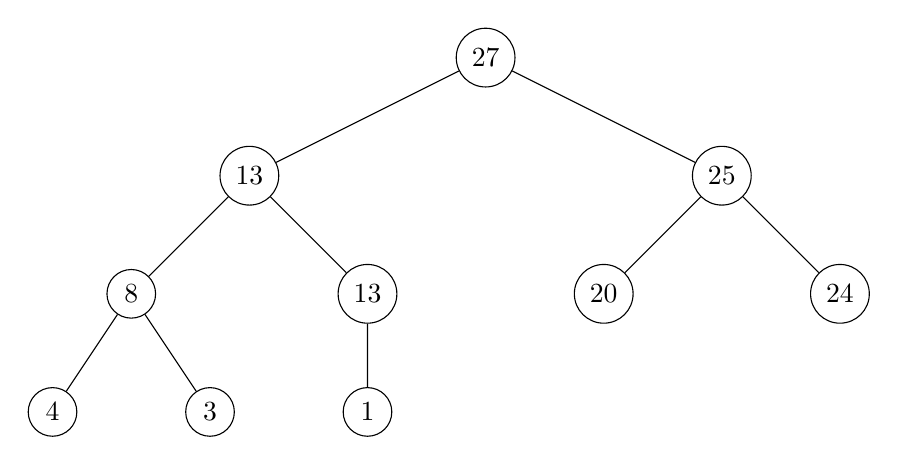
\begin{tikzpicture}[level/.style={sibling distance=60mm/#1}]
\node [circle,draw] (z){$27$}
  child {node [circle,draw] (a) {$13$}
    child {node [circle,draw] (b) {$8$}
      child {node [circle,draw] (d) {$4$}}
      child {node [circle,draw] (e) {$3$}}
    }
    child {node [circle,draw] (g) {$13$}
      child {node [circle,draw] (h) {$1$}}
    }
  }
  child {node [circle,draw] (j) {$25$}
    child {node [circle,draw] (k) {$20$}}
  child {node [circle,draw] (l) {$24$}}
};
\end{tikzpicture}
\end{center}

힙의 노드마다 번호를 매길 수 있는데, 루트에 0부터 매기기 시작해서
위부터 아래로, 왼쪽에서 오른쪽으로 매길 수 있다.  위 예제는 다음 배열
\texttt{A}와 같이 표현할 수 있다:

\begin{center}
\begin{tabular}{|l|l|l|l|l|l|l|l|l|l|l|}
\hline
$i$ & 0 & 1 & 2 & 3 & 4 & 5 & 6 & 7 & 8 & 9\\
\hline
$\texttt{A}(i)$ & 27 & 13 & 25 & 8 & 13 & 20 & 24 & 4 & 3 & 1\\
\hline
\end{tabular}
\end{center}
\noindent 이런 경우, $i$번의 두 자식은 $2i+1$과 $2i+2$가
된다. (확인해보라!)  이제부터 $heap(\texttt{A}, n)$을, 배열
$\texttt{A}$가 길이 $n$ 짜리 힙임을 의미한다고 하자.

힙에서 가장 큰 값을 꺼내는 연산 \texttt{pop(A: int[10], n: int): int $\times$
  int[10]}은 다음 명세를 만족해야 한다:
\begin{align*}
  & \inv{\texttt{A: int[10]} \land heap(\texttt{A}, \texttt{n}) \land \texttt{n}>0} \\
  \texttt{10:}& \texttt{(x, B) := pop(A, n)} \\
  & \inv{\texttt{B: int[10]} \land heap(\texttt{B}, \texttt{n}-1) \land (\mbox{\texttt{x}가 \texttt{A[0, n-1]}에서 가장 큰 값})}
\end{align*}

다음과 같이 \texttt{pop}을 정의하면 명세를 만족한다는 것이 알려졌다:
\begin{align*}
\texttt{10:}& \texttt{pop(A: int[10], n: int): int $\times$ int[10] :=} \\
\texttt{11:}& \ \ \texttt{B := A, x := B(0), B(0) := B(n-1), i := 0} \\
\texttt{12:}& \ \ \texttt{while (i * 2 + 1 < n - 1) \{} \\
\texttt{13:}& \ \ \ \ \texttt{j := i * 2 + 1} \\
\texttt{14:}& \ \ \ \ \texttt{if (j + 1 < n - 1 \&\& B(j) < B(j+1)) \{} \\
\texttt{15:}& \ \ \ \ \ \ \texttt{++j} \\
\texttt{16:}& \ \ \ \ \texttt{\}} \\
\texttt{17:}& \ \ \ \ \texttt{if (B(i) < B(j)) \{} \\
\texttt{18:}& \ \ \ \ \ \ \texttt{swap(B(i), B(j)), i := j} \\
\texttt{19:}& \ \ \ \ \texttt{\} else \{} \\
\texttt{20:}& \ \ \ \ \ \ \texttt{break} \\
\texttt{21:}& \ \ \ \ \texttt{\}} \\
\texttt{22:}& \ \ \texttt{\}} \\
\texttt{23:}& \ \ \texttt{return (x, B)}
\end{align*}

\begin{exercise}
  \texttt{pop} 함수에 적절한 불변식을 넣어서, 주어진 명세를 만족함을
  보여라.
\end{exercise}
\begin{homework}
  힙의 다른 연산들 (초기화, 삽입)에 대해서도 명세를 밝혀라.  명세를
  만족하는 함수를 정의하고, 적절한 불변식을 넣어서, 명세를 만족함을
  보여라.
\end{homework}

\section{마치며}
2003년 KOI 중등부 1번 문제는 그래프의 최단거리를 구하는 문제였다.  나는
아는 문제가 나와서 기뻐하며 다음과 같이 Floyd-Warshall 알고리즘을
작성했다:
\begin{align*}
& \texttt{for \texttt{i} := 1 to n do} \\
& \ \ \texttt{for \texttt{j} := 1 to n do} \\
& \ \ \ \ \texttt{for \texttt{k} := 1 to n do} \\
& \ \ \ \ \ \ \texttt{if (d[i][k] > d[i][j] + d[j][k])} \\
& \ \ \ \ \ \ \ \ \texttt{d[i][k] := d[i][j] + d[j][k]}
\end{align*}
하지만 위 알고리즘은 \emph{틀렸다}.  올바른 알고리즘은, 루프를
\emph{\texttt{k}부터} 돌려야 한다:
\begin{align*}
& \texttt{for \texttt{k} := 1 to n do} \\
& \ \ \texttt{for \texttt{i} := 1 to n do} \\
& \ \ \ \ \texttt{for \texttt{j} := 1 to n do} \\
& \ \ \ \ \ \ \texttt{if (d[i][k] > d[i][j] + d[j][k])} \\
& \ \ \ \ \ \ \ \ \texttt{d[i][k] := d[i][j] + d[j][k]}
\end{align*}
내가 이 문제를 틀렸던 까닭은, 알고리즘이 왜 맞는지에 대한 이해 없이,
무조건 알고리즘을 외워서 대회에서 써먹으려고 했기 때문이다.  불변식을
써서 알고리즘이 왜 맞는지 체계적으로 이해해야만, 대회에서 문제를 만났을
때 자신 있게 알고리즘을 적용할 수 있다.  이는 쉬운 문제나 어려운 문제,
그리고 궁극적으로 현업에서 만날 문제에 이르기까지 변치 않는 중요한
원칙이다.  여러분들은 불변식을 숙지해서, 내가 대회에서 저질렀던
어이없는 실수를 저지르지 않길 바란다.

\begin{homework}
  Floyd-Warshall 알고리즘의 명세를 밝히고, 적절한 불변식을 넣어 명세가
  옳음을 보여라.  힌트: $\texttt{k}$는 경로가 방문하는 노드의 수와
  관련이 있다.
\end{homework}
\begin{homework}
  2014년 KOI 문제를 천천히 읽어보고, 수학적으로 명확한 명세를 밝혀라.
  명세에 대한 답안을 작성하고, 적절한 불변식을 넣어 답안이 명세에 대해
  옳음을 보여라.
\end{homework}

\end{document}
